\documentclass[12pt]{article}

\usepackage[margin=1in]{geometry}
\usepackage[T1]{fontenc}
\usepackage{lmodern}
\usepackage{microtype}
\usepackage{amsmath,amssymb,mathtools}
\usepackage{booktabs}
\usepackage{float}
\usepackage{enumitem}
\usepackage{setspace}
\usepackage{xcolor}
\usepackage{tikz}
\usepackage{hyperref}
\usepackage{xurl}

\hypersetup{
  colorlinks=true,
  linkcolor=black,
  citecolor=black,
  urlcolor=blue,
  pdftitle={Schwarzschild Tides: Geodesic Deviation, Shape Change, and Curvature},
  pdfauthor={Light-Meter Physics},
  pdfsubject={Geodesic deviation and curvature in the Schwarzschild spacetime},
  pdfkeywords={tidal forces, geodesic deviation, Schwarzschild spacetime, Kretschmann scalar}
}

\onehalfspacing
\widowpenalty=10000
\clubpenalty=10000
\definecolor{ink}{HTML}{172E3D}
\definecolor{teal}{HTML}{126D77}
\definecolor{rust}{HTML}{B1533E}
\definecolor{pale}{HTML}{A9B7BF}

\title{Schwarzschild Tides:\\
Geodesic Deviation, Shape Change, and Curvature}
\author{Light-Meter Physics}
\date{}

\begin{document}

\maketitle

\begin{abstract}
A small cloud of freely falling probes near a nonrotating spherical mass is stretched radially and compressed in two transverse directions. This manuscript derives that pattern using geodesic deviation in the Schwarzschild vacuum exterior. In a local orthonormal frame carried by a radially falling observer, the relative-acceleration coefficients are $2GM/r^3$ radially and $-GM/r^3$ in each transverse direction. With the characteristic times $\tau_g=GM/c^3$ and $t_r=r/c$, the shared scale is $\tau_g/t_r^3=GM/r^3$. The tidal matrix is trace-free, so an initially comoving infinitesimal sphere has zero instantaneous volume acceleration even as it begins to change shape. The Schwarzschild Kretschmann scalar is $K=48[GM/(c^2r^3)]^2$; counting the orthonormal Riemann components explains the factor $48$ and lets this invariant recover the same tidal scale in this geometry. At the horizon, both the tidal scale and $K$ are finite, with their values decreasing as the black-hole mass increases. These results are specific to the stated spacetime and observer setup, not a new law of gravity.
\end{abstract}

\noindent\textbf{Keywords:} tidal forces, geodesic deviation, Schwarzschild spacetime, curvature invariant, black-hole horizon

\section{Introduction}
\label{sec:introduction}

An ideal accelerometer on a freely falling probe reads zero, yet nearby freely falling probes can accelerate relative to one another. Gravity can accelerate the center of a freely falling body without producing a force that the body locally feels; neighboring parts follow slightly different geodesics. Their relative acceleration is a tidal effect, described in general relativity by geodesic deviation \cite{TongGR,HamiltonGR}.

For a small cloud falling radially outside a spherical, nonrotating mass, the local pattern is simple: one principal direction stretches, while two perpendicular directions squeeze. In vacuum the Ricci tensor vanishes, but the Riemann curvature and the tidal effects do not. This makes the example a useful way to distinguish a vanishing Ricci trace from vanishing spacetime curvature.

The discussion derives the local relative accelerations first and then follows their immediate effect on the shape and volume of a small sphere. It next counts the orthonormal-frame curvature components that contribute to the Kretschmann scalar, explaining why the coefficient is $48$. Throughout, $r$ is the Schwarzschild areal radius, distances between nearby probes are local proper separations, and the central observer's proper time is denoted by $\tau$. No new symbol is introduced for the common factor $\tau_g/t_r^3$.

\section{Schwarzschild model and notation}
\label{sec:model}

Consider the vacuum exterior of a spherical, nonrotating source of mass $M$. In Schwarzschild coordinates the metric is
\begin{equation}
  ds^2=-F(r)c^2dt^2+F(r)^{-1}dr^2
      +r^2\left(d\theta^2+\sin^2\theta\,d\phi^2\right),
  \qquad
  F(r)=1-\frac{2GM}{rc^2}.
  \label{eq:schwarzschild-metric}
\end{equation}
The coordinate $r$ is the areal radius: a sphere at fixed $r$ has area $4\pi r^2$. For a Schwarzschild black hole, the event-horizon radius is $r_H=2GM/c^2$. A spherical star with surface radius $R_*>2GM/c^2$ has the same Schwarzschild vacuum exterior for $r>R_*$, but no horizon lies in that exterior; the horizon evaluations below apply only to the black-hole case \cite{TongGR}. Choose a freely falling central observer on a radial geodesic and a parallel-transported orthonormal tetrad along its worldline, with $e_{\hat 0}=u/c$. The spatial axes are radial and transverse. The connecting vector $\xi^{\hat i}$ measures local proper separation, and initially comoving probes satisfy $D\xi^{\hat i}/D\tau=0$ at release. This condition does not require the central observer to be at rest in Schwarzschild coordinates \cite{HamiltonGR}.

Use the gravitational time and radius-time
\begin{equation}
  \tau_g\equiv\frac{GM}{c^3},
  \qquad
  t_r\equiv\frac{r}{c}.
  \label{eq:time-definitions}
\end{equation}
These are scales formed from the mass and areal radius, not clock readings. Dividing $\tau_g$ by $t_r^3$ gives the coefficient that appears in the tidal equations:
\begin{equation}
  \frac{\tau_g}{t_r^3}=\frac{GM}{r^3},
  \qquad
  \left[\frac{\tau_g}{t_r^3}\right]=\mathrm{s^{-2}}.
  \label{eq:shared-scale}
\end{equation}
For comparison, a Newtonian circular test-particle orbit at the same radius has $(2\pi/T_S)^2=GM/r^3$, where $T_S$ is its full period \cite{NASAFlight}. This is the same inverse-cube scale, but an orbital rate and a tidal relative acceleration are distinct physical quantities. The time coordinate $t$ in Eq.~\eqref{eq:schwarzschild-metric} is not the proper time $\tau$ of the falling observer.

\section{Newtonian intuition for the three directions}
\label{sec:newtonian}

In the Newtonian point-source model, the signed radial acceleration of a freely falling test body is $a_r=-GM/r^2$, with outward radial direction positive. Two initially comoving probes separated by a small radial displacement $\xi^{\hat r}$ therefore have, to first order,
\begin{equation}
  \Delta a^{\hat r}
  \simeq\frac{d}{dr}\left(-\frac{GM}{r^2}\right)\xi^{\hat r}
  =\frac{2GM}{r^3}\,\xi^{\hat r}.
  \label{eq:newtonian-radial}
\end{equation}
The outer probe accelerates inward less strongly, so their radial separation grows. For a small transverse displacement, the inward acceleration vectors point in slightly different directions. Their transverse difference is
\begin{equation}
  \Delta\boldsymbol a_{\perp}
  \simeq-\frac{GM}{r^3}\,\boldsymbol\xi_{\perp},
  \label{eq:newtonian-transverse}
\end{equation}
which tends to reduce the transverse separation \cite{OregonTides}.

These Newtonian expressions motivate the pattern and match the Schwarzschild coefficients in the radial freely falling frame considered here. They are not the relativistic derivation: that follows from the curvature tensor and geodesic deviation. The matching coefficients should not be read as making the Newtonian and relativistic descriptions identical in general.

\section{Relativistic tidal acceleration}
\label{sec:geodesic-deviation}

Let $\xi^{\hat i}$ be the spatial separation between the central geodesic and a neighboring geodesic. Adopt a Riemann-tensor convention for which geodesic deviation is
\begin{equation}
  \frac{D^2\xi^\mu}{D\tau^2}
  =-R^\mu{}_{\alpha\nu\beta}
      u^\alpha\xi^\nu u^\beta,
  \label{eq:geodesic-deviation}
\end{equation}
where $u^\mu$ is the central observer's four-velocity. In the parallel-transported orthonormal frame, $u^{\hat\alpha}=(c,0,0,0)$, and covariant proper-time derivatives of the spatial components reduce to ordinary derivatives. A short derivation identifies the tidal operator. For radial Schwarzschild motion, the conserved dimensionless energy is $E=F(r)\,dt/d\tau$. Normalization of the four-velocity gives
\begin{equation}
  \dot r^{\,2}=c^2\bigl(E^2-F(r)\bigr),
  \qquad
  \ddot r=-\frac{c^2}{2}\frac{dF}{dr}=-\frac{GM}{r^2},
  \label{eq:radial-geodesic}
\end{equation}
where dots denote derivatives with respect to $\tau$. Rotating this radial geodesic by a fixed infinitesimal angle $\delta\theta$ gives a neighboring geodesic with transverse proper separation $\xi_\perp=r\,\delta\theta$, so $\ddot\xi_\perp/\xi_\perp=\ddot r/r=-GM/r^3$. Spherical symmetry gives the same eigenvalue in the other transverse direction. This rotated-geodesic variation identifies the transverse tidal operator; if the central observer is falling, it generally has nonzero initial relative velocity $\dot\xi_\perp=\dot r\,\delta\theta$, so it is not the initially comoving cloud considered in the next section. In vacuum $R_{\hat 0\hat 0}=0$, making the trace of the geodesic-deviation operator zero and fixing the radial eigenvalue at $+2GM/r^3$ \cite{TongGR,OregonTides}. Evaluation of the Schwarzschild curvature components therefore gives
\begin{equation}
  \frac{D^2\xi^{\hat i}}{D\tau^2}
  =-c^2R^{\hat i}{}_{\hat 0\hat j\hat 0}\,\xi^{\hat j}
  =\frac{\tau_g}{t_r^3}
    \begin{pmatrix}
      2&0&0\\
      0&-1&0\\
      0&0&-1
    \end{pmatrix}^{\hat i}{}_{\hat j}
    \xi^{\hat j}.
  \label{eq:tidal-matrix}
\end{equation}
Thus
\begin{align}
  \frac{D^2\xi^{\hat r}}{D\tau^2}
    &=2\frac{\tau_g}{t_r^3}\,\xi^{\hat r},\\
  \frac{D^2\xi^{\hat\theta}}{D\tau^2}
    &=-\frac{\tau_g}{t_r^3}\,\xi^{\hat\theta},\\
  \frac{D^2\xi^{\hat\phi}}{D\tau^2}
    &=-\frac{\tau_g}{t_r^3}\,\xi^{\hat\phi}.
  \label{eq:tidal-components}
\end{align}
The positive radial coefficient describes stretching; the negative transverse coefficients describe squeezing. The acceleration is relative acceleration between neighboring geodesics, not a proper force acting on either freely falling probe. A different Riemann-sign convention changes the signs assigned to curvature components, but not this physical stretching-and-squeezing result when the geodesic-deviation convention is changed consistently \cite{HamiltonGR}.

\begin{figure}[tb]
  \centering
  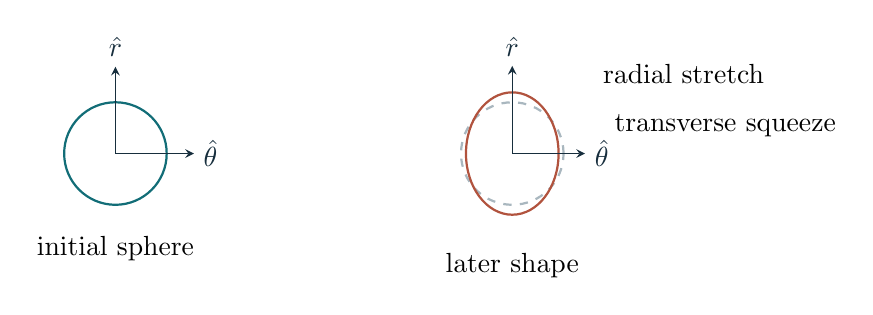
\begin{tikzpicture}[>=stealth,scale=1.05]
    \draw[teal,thick] (-2.4,0) circle[radius=0.62];
    \draw[->,ink] (-2.4,0)--(-2.4,1.05)
      node[above] {$\hat r$};
    \draw[->,ink] (-2.4,0)--(-1.45,0)
      node[right] {$\hat\theta$};
    \node[below=8pt] at (-2.4,-0.62) {initial sphere};

    \draw[dashed,pale,thick] (2.4,0) circle[radius=0.62];
    \draw[rust,thick] (2.4,0) ellipse[x radius=0.56,y radius=0.74];
    \draw[->,ink] (2.4,0)--(2.4,1.06)
      node[above] {$\hat r$};
    \draw[->,ink] (2.4,0)--(3.28,0)
      node[right] {$\hat\theta$};
    \node[below=8pt] at (2.4,-0.82) {later shape};
    \node[anchor=west] at (3.38,0.96) {radial stretch};
    \node[right=20pt] at (2.85,0.34) {transverse squeeze};
  \end{tikzpicture}
  \caption{Schematic local cross-section of an initially spherical cloud and its later shape. The dashed circle marks the release size. The drawing exaggerates the leading displacements and shows one of the two equivalent transverse directions; it is not a finite-time volume calculation.}
  \label{fig:tidal-shape}
\end{figure}

\section{Shape change and initial volume acceleration}
\label{sec:volume}

Take the three principal semiaxes of an infinitesimal sphere to be $L_{\hat r}$, $L_{\hat\theta}$, and $L_{\hat\phi}$. Dots denote derivatives with respect to the central observer’s proper time. At release, let all three axes have length $L$ and let their first derivatives vanish. The initial comoving condition is $D\xi^{\hat i}/D\tau=0$ at release; it does not mean that the central observer is initially at rest. Using the tidal matrix in Eq.~\eqref{eq:tidal-matrix} then gives
\begin{equation}
  \left.
  \left(
    \frac{\ddot L_{\hat r}}{L_{\hat r}},
    \frac{\ddot L_{\hat\theta}}{L_{\hat\theta}},
    \frac{\ddot L_{\hat\phi}}{L_{\hat\phi}}
  \right)
  \right|_{\rm release}
  =\frac{\tau_g}{t_r^3}(2,-1,-1),
  \label{eq:axis-accelerations}
\end{equation}
where the coefficient is evaluated at the central observer's release radius. To quadratic order in a short proper-time interval $\Delta\tau$, the radial semiaxis grows by the fractional amount $(\tau_g/t_r^3)(\Delta\tau)^2$, while each transverse semiaxis decreases by half that fractional amount.

The local volume is proportional to the product of the three semiaxes. Since their first derivatives vanish at release,
\begin{equation}
  \left.\frac{\dot V}{V}\right|_{\rm release}=0,\\
  \left.\frac{\ddot V}{V}\right|_{\rm release}
  =\left.\left(
    \frac{\ddot L_{\hat r}}{L_{\hat r}}
    +\frac{\ddot L_{\hat\theta}}{L_{\hat\theta}}
    +\frac{\ddot L_{\hat\phi}}{L_{\hat\phi}}
  \right)\right|_{\rm release}
  =\frac{\tau_g}{t_r^3}(2-1-1)=0.
  \label{eq:volume-acceleration}
\end{equation}
The vacuum tidal trace remains zero along the trajectory. At release the vanishing relative velocities make both $\dot V$ and $\ddot V$ zero, even as the axis accelerations change the cloud's shape. At later times the product rule gives
\begin{equation}
  \frac{\ddot V}{V}=\sum_i\frac{\ddot L_i}{L_i}
  +2\sum_{i<j}\frac{\dot L_i}{L_i}\frac{\dot L_j}{L_j},
  \label{eq:volume-product-rule}
\end{equation}
so products of the fractional axis velocities can change the volume even when the tidal trace is zero. Vacuum does not mean zero Riemann curvature or zero tidal acceleration \cite{TongGR}.

\section{Counting the curvature components}
\label{sec:curvature-components}

In the local orthonormal frame, there are six distinct diagonal pair components $R_{\hat a\hat b\hat a\hat b}$, with no sum on the indices. Their magnitudes are \cite{HamiltonGR}:
\begin{center}
\small
\begin{tabular}{@{}p{0.42\linewidth}p{0.52\linewidth}@{}}
  \toprule
  Orthonormal pair & Magnitude of $R_{\hat a\hat b\hat a\hat b}$ (no sum) \\
  \midrule
  $(\hat 0\hat r)$ and $(\hat\theta\hat\phi)$
    & $2GM/(c^2r^3)$ \\
  $(\hat 0\hat\theta)$, $(\hat 0\hat\phi)$,
  $(\hat r\hat\theta)$, and $(\hat r\hat\phi)$
    & $GM/(c^2r^3)$ \\
  \bottomrule
\end{tabular}
\end{center}
With the Riemann convention of Eq.~\eqref{eq:geodesic-deviation}, a signed check from the metric gives the normalized components $(-2,+1,+1,+2,-1,-1)$ for the ordered pairs $(\hat 0\hat r,\hat 0\hat\theta,\hat 0\hat\phi,\hat\theta\hat\phi,\hat r\hat\phi,\hat r\hat\theta)$, in units of $GM/(c^2r^3)$. Reversing either antisymmetric pair generates four arrangements for each diagonal pair component: $abab$, $abba$, $baab$, and $baba$. Exchanging the two index pairs adds no fifth arrangement. In these nonzero components there are zero or two time indices, so all four terms contribute positively to the contraction $R_{\alpha\beta\gamma\delta}R^{\alpha\beta\gamma\delta}$. The result is
\begin{align}
  K&\equiv R_{\alpha\beta\gamma\delta}
                 R^{\alpha\beta\gamma\delta}\\
   &=4\left[
      2\left(\frac{2GM}{c^2r^3}\right)^2
      +4\left(\frac{GM}{c^2r^3}\right)^2
     \right]
    =48\left(\frac{GM}{c^2r^3}\right)^2.
  \label{eq:kretschmann}
\end{align}
The factor $4$ counts the four arrangements of each component; the bracket contains two components of magnitude $2GM/(c^2r^3)$ and four of magnitude $GM/(c^2r^3)$. The contraction therefore has 24 nonzero ordered terms and agrees with the Schwarzschild Kretschmann scalar computed directly from the metric \cite{TongGR}.

\section{The invariant and the local tidal scale}
\label{sec:invariant}

Substituting Eq.~\eqref{eq:shared-scale} into Eq.~\eqref{eq:kretschmann} gives
\begin{equation}
  K=\frac{48}{c^4}\left(\frac{\tau_g}{t_r^3}\right)^2,
  \qquad
  \frac{\tau_g}{t_r^3}=c^2\sqrt{\frac{K}{48}}
  \quad (M>0).
  \label{eq:invariant-scale}
\end{equation}
The square root selects the positive-mass branch. The Kretschmann scalar has units $\mathrm{m^{-4}}$, so $c^2\sqrt{K/48}$ has units $\mathrm{s^{-2}}$, as required for the coefficient in Eq.~\eqref{eq:tidal-matrix}. In this Schwarzschild model, the scalar determines the magnitude of the displayed tidal coefficient. It does not generally determine the full tidal tensor in an arbitrary spacetime: a scalar contraction discards directional information, and different geometries can have the same scalar value.

\section{Horizon values and mass scaling}
\label{sec:horizon}

For a Schwarzschild black hole,
\begin{equation}
  r_H=\frac{2GM}{c^2},
  \qquad
  t_{r,H}\equiv\frac{r_H}{c}=2\tau_g.
  \label{eq:horizon-radius}
\end{equation}
Evaluating the characteristic scale and curvature invariant at the horizon gives
\begin{align}
  \left.\frac{\tau_g}{t_r^3}\right|_{r_H}
    &=\frac{1}{8\tau_g^2},\\
  K_H
    &=\frac{12}{r_H^4}
     =\frac{3}{4c^4\tau_g^4}.
  \label{eq:horizon-values}
\end{align}
Both are finite in a regular freely falling frame at the black-hole horizon. There the radial relative acceleration per unit radial separation is $+1/(4\tau_g^2)$, while each transverse relative acceleration per unit transverse separation is $-1/(8\tau_g^2)$. For equal small proper separations, each squeeze has half the magnitude of the radial stretch. Since $\tau_g$ is proportional to $M$, the tidal coefficient at each hole's own horizon scales as $M^{-2}$, while $K_H$ scales as $M^{-4}$. Thus, for a 10:1 mass ratio evaluated at each black hole's own horizon, the heavier hole has one hundredth the tidal acceleration for a fixed small proper separation and one ten-thousandth the Kretschmann scalar \cite{TongGR,HamiltonGR}.

The finiteness of these scalars distinguishes the horizon from the central Schwarzschild curvature singularity, where $K$ diverges as $r\to0$. Schwarzschild coordinates become singular at the horizon, but the finite curvature invariant and the local freely falling description show that this coordinate behavior is not a divergence in the local tidal field.

\section{A comparison with plane-wave tides}
\label{sec:plane-wave}

A linearized vacuum plane gravitational wave provides a brief contrast. In a suitable local transverse basis, its instantaneous tidal-acceleration matrix has two opposite transverse eigenvalues and a zero eigenvalue along the propagation direction, with the trace again vanishing \cite{TongGR}. The Schwarzschild eigenvalue pattern is instead proportional to $(2,-1,-1)$: it has one radial stretch and two transverse squeezes. The comparison illustrates that vacuum tidal matrices can be trace-free while having different shapes. It does not identify the two geometries or imply that they share the same curvature invariant.

\section{Interpretive limits and conclusion}
\label{sec:conclusion}

The result assumes a spherical, nonrotating Schwarzschild vacuum and an infinitesimal cloud of freely falling probes. Matter in the region sampled, departures from spherical symmetry, or rotation can change the tidal field; finite separations can require higher spatial derivatives. A spherical star with a vacuum exterior has the same Schwarzschild field as a black hole of equal mass at any shared exterior radius, but the horizon results apply only to a black hole \cite{TongGR}. The Newtonian gradient in Sec.~\ref{sec:newtonian} is a useful guide, but the relativistic result follows from geodesic deviation, not from applying Newton's law inside a black hole.

For the stated observer and geometry, geodesic deviation gives one stretching and two squeezing directions, with the shared coefficient $\tau_g/t_r^3=GM/r^3$. Its trace vanishes, explaining the zero instantaneous volume acceleration of an initially comoving sphere without implying that its shape or later volume is unchanged. Counting the orthonormal Riemann components gives the factor $48$ in the Kretschmann scalar and relates that scalar back to the local tidal scale. The horizon values remain finite and decrease with increasing mass. Each step is a result of the Schwarzschild model, not a new gravitational law.

\appendix

\section{Dimensional and algebraic checks}
\label{app:checks}

The characteristic times and curvature scale satisfy
\begin{equation}
  \left[\frac{\tau_g}{t_r^3}\right]=\mathrm{s^{-2}},
  \qquad
  \left[\frac{GM}{c^2r^3}\right]=\mathrm{m^{-2}},
  \qquad
  [K]=\mathrm{m^{-4}}.
  \label{eq:dimensions}
\end{equation}
Using $t_r=r/c$ and $\tau_g=GM/c^3$ directly verifies
\begin{equation}
  \frac{1}{c^4}\left(\frac{\tau_g}{t_r^3}\right)^2
  =\left(\frac{GM}{c^2r^3}\right)^2,
  \qquad
  \left.\frac{\tau_g}{t_r^3}\right|_{r_H}
  =\frac{\tau_g}{(2\tau_g)^3}
  =\frac{1}{8\tau_g^2}.
  \label{eq:checks}
\end{equation}
These identities check the units and the horizon substitution independently of the curvature-component count.

\section{Numerical horizon comparison}
\label{app:numerical-comparison}

For the stellar-mass example, take $M_{10}=10M_\odot$. For Sagittarius A*, adopt the stellar-orbit mass estimate $M_{\mathrm{Sgr\,A^*}}=4.297\times10^6M_\odot$ \cite{GravitySgrA}. Using $GM_\odot/c^3\simeq4.92564\,\mu\mathrm{s}$ gives
\begin{align}
  \tau_{g,10}
    &=(4.92564\,\mu\mathrm{s})(10)
      =49.2564\,\mu\mathrm{s}\simeq49.3\,\mu\mathrm{s},\\
  \tau_{g,\mathrm{Sgr\,A^*}}
    &=(4.92564\,\mu\mathrm{s})(4.297\times10^6)
      =21.1655\,\mathrm{s}\simeq21.2\,\mathrm{s}.
  \label{eq:numerical-mass-times}
\end{align}
At the Schwarzschild horizon, the relevant relations are
\begin{equation}
  r_H=2c\tau_g,
  \qquad
  t_{r,H}=\frac{r_H}{c}=2\tau_g,
  \qquad
  \Delta a^{\hat r}(\ell)\simeq\frac{\ell}{4\tau_g^2},
  \qquad
  K_H=\frac{3}{4c^4\tau_g^4}.
  \label{eq:numerical-horizon-relations}
\end{equation}
Here $\Delta a^{\hat r}(\ell)$ is the leading-order radial relative-acceleration difference across a small proper separation $\ell$, obtained from the radial eigenvalue in Eq.~\eqref{eq:horizon-values}. For $\ell=2\,\mathrm{m}$, the acceleration calculations are
\begin{align}
  \Delta a^{\hat r}_{10}(2\,\mathrm{m})
    &=\frac{2\,\mathrm{m}}{4(49.2564\times10^{-6}\,\mathrm{s})^2}
      \simeq2.06\times10^8\,\mathrm{m\,s^{-2}},\\
  \Delta a^{\hat r}_{\mathrm{Sgr\,A^*}}(2\,\mathrm{m})
    &=\frac{2\,\mathrm{m}}{4(21.1655\,\mathrm{s})^2}
      \simeq1.12\times10^{-3}\,\mathrm{m\,s^{-2}}.
  \label{eq:numerical-horizon-values}
\end{align}
Substituting the same mass timescales into the horizon-radius, radius-time, and Kretschmann formulas in Eq.~\eqref{eq:numerical-horizon-relations} gives the remaining rounded values in Table~\ref{tab:numerical-horizon-comparison}. The Sagittarius A* column applies the Schwarzschild formulas as a mass-scaling illustration; it is not a spin-dependent Kerr calculation.

\begin{table}[H]
  \centering
  \small
  \begin{tabular}{@{}p{0.41\linewidth}p{0.23\linewidth}p{0.30\linewidth}@{}}
    \toprule
    Quantity at the horizon & $10\,M_\odot$ & Sagittarius A* \\
    \midrule
    Mass timescale $\tau_g=GM/c^3$
      & $49.3\,\mu\mathrm{s}$ & $21.2\,\mathrm{s}$ \\
    Horizon radius $r_H=2c\tau_g$
      & $29.5\,\mathrm{km}$ & $12.7$ million $\mathrm{km}$ \\
    Radius in light-seconds $t_{r,H}=r_H/c$
      & $98.5\,\mu\mathrm{s}$ & $42.3\,\mathrm{s}$ \\
    Radial tidal acceleration across $2\,\mathrm{m}$
      & $2.06\times10^8\,\mathrm{m\,s^{-2}}$
      & $1.12\times10^{-3}\,\mathrm{m\,s^{-2}}$ \\
    Kretschmann scalar $K_H$
      & $1.58\times10^{-17}\,\mathrm{m^{-4}}$
      & $4.63\times10^{-40}\,\mathrm{m^{-4}}$ \\
    \bottomrule
  \end{tabular}
  \caption{Horizon quantities for a $10\,M_\odot$ Schwarzschild black hole and a Schwarzschild mass-scaling model using the adopted Sagittarius A* mass. The tidal-acceleration entry is the leading-order relative-acceleration difference across a $2\,\mathrm{m}$ local proper separation.}
  \label{tab:numerical-horizon-comparison}
\end{table}

\clearpage

Within the Schwarzschild model, $r_H=2GM/c^2\propto M$, while the radial tidal relative-acceleration coefficient at the horizon, $1/(4\tau_g^2)$, scales as $M^{-2}$. Thus a more massive black hole has a larger horizon and gentler local tides at crossing. For the $2\,\mathrm{m}$ separation in Table~\ref{tab:numerical-horizon-comparison}, the radial acceleration difference is about $2.1\times10^7g_\oplus$ at the $10\,M_\odot$ horizon and $1.1\times10^{-4}g_\oplus$ at the Sagittarius A* horizon, taking $g_\oplus\simeq9.81\,\mathrm{m\,s^{-2}}$. Each freely falling probe's ideal accelerometer reads zero; the tidal signal is the relative acceleration inferred from how their separation evolves.

\begin{thebibliography}{9}
\small
\setstretch{1.0}
\raggedright
\urlstyle{same}

\bibitem{TongGR}
D. Tong,
\emph{General Relativity},
lecture notes, University of Cambridge, Secs.~3.3.4, 5.2.2, 6.1.1, and 6.1.2, including Eq.~(6.258),
available at \href{https://www.damtp.cam.ac.uk/user/tong/gr/grhtml/}{Cambridge General Relativity Notes}.

\bibitem{HamiltonGR}
A. J. S. Hamilton,
\emph{General Relativity, Black Holes, and Cosmology},
Exercise~11.10 and Eqs.~(11.101)--(11.103),
JILA, University of Colorado Boulder,
available at \href{https://jila.colorado.edu/~ajsh/courses/astr5770_21/grbook.pdf}{JILA General Relativity Notes}.

\bibitem{GravitySgrA}
GRAVITY Collaboration,
``Mass distribution in the Galactic Center based on interferometric astrometry of multiple stellar orbits,''
\emph{Astronomy \& Astrophysics} \textbf{657}, L12 (2022),
available at \href{https://doi.org/10.1051/0004-6361/202142465}{doi:10.1051/0004-6361/202142465}.

\bibitem{NASAFlight}
NASA,
\emph{Basics of Space Flight},
Chapter~3, ``Gravity \& Mechanics,''
available at \href{https://science.nasa.gov/learn/basics-of-space-flight/chapter3-3/}{NASA Basics of Space Flight}.

\bibitem{OregonTides}
Oregon State University,
``Tidal Forces,''
Chapter~6, Geodesic Deviation,
available at \href{https://sites.science.oregonstate.edu/physics/coursewikis/GGR/book/ggr/tidal.html}{Oregon State University General Relativity Notes}.

\end{thebibliography}

\end{document}